\documentclass{report}
\usepackage{listings}
\usepackage{graphicx}
\def\weight{0.7}

\title{Report on CNN/Scattering classification comparison}
\author{Alberto Carli \and Gabriele Roncolato \and Leonardo Zecchin }
\date{}

\begin{document}
\maketitle
\tableofcontents
\pagebreak

\chapter{Introduction}
This document illustrates the project valid for the Visual Intelligence class of the academic year 2022/2023. \\
The assignment tests the knowledge gained in class by applying signal analysis methods, in particular we classified signals by using \textbf{Convolutional Neural Networks} and wavelet theory, specifically  \textbf{Wavelet Scattering}. \\
In this project we implemented the code necessary to classify a given dataset first by training and testing a CNN, then by applying the Wavelet Scattering Transform and training a NN with the extracted features.
Finally we compared the results obtained with these two methods in terms of accuracy against how many epochs were used to train the classifiers. \\
For the entire project, we followed the guidelines given during the laboratory lectures.


\chapter{Objectives}
The goal of this project is to explore the use of scattering transforms to improve the performance of neural networks on a given dataset.\\
Specifically, we aimed to compare the performance of a CNN trained on the original dataset to a NN trained on the scattering decomposition of the data.\\

We then visualized the filters learned by the CNN and compared them to the ones applied by the scattering transform to gain insight into the types of features that were extracted. 
By accomplishing these objectives we hoped to gain a better understanding of how the CNN learns which features to extract.

\chapter{Dataset}
We used a dataset consisting of 128x128 RGB images divided into two categories: dogs and flowers. There are 1600 pictures of dogs and 1387 pictures of flowers.
We converted everything to grayscale with each class n its specific folder and every file numbered.

\chapter{Framework}
\section{Convolutional Neural Network}
\subsection{What is a CNN}
A Convolutional Neural Network (\textbf{CNN}) is a type of deep learning algorithm commonly used for image recognition and computer vision tasks. It is designed to automatically learn and extract relevant features from input images through convolutional and pooling layers, followed by fully connected layers that produce output predictions. \\
The \texttt{CNN\_128x128} architecture consists of four \textbf{convolutional} layers and three fully connected layers. The first layer takes an input image with \texttt{input\_channel} number of channels, and the output of the last layer is a vector with \texttt{num\_classes} elements representing the probability of each class.

\subsection{Architecture}
\begin{lstlisting}[language=bash]
CNN_128x128(
    (conv1): Conv2d(1, 16, kernel_size=(7, 7), stride=(2, 2), padding=(1, 1))
    (conv2): Conv2d(16, 32, kernel_size=(5, 5), stride=(2, 2), padding=(1, 1))
    (conv3): Conv2d(32, 64, kernel_size=(3, 3), stride=(2, 2), padding=(1, 1))
    (batchnorm1): BatchNorm2d(16, eps=1e-05, momentum=0.1, affine=True, track_running_stats=True)
    (batchnorm2): BatchNorm2d(32, eps=1e-05, momentum=0.1, affine=True, track_running_stats=True)
    (batchnorm3): BatchNorm2d(64, eps=1e-05, momentum=0.1, affine=True, track_running_stats=True)
    (drop1): Dropout(p=0.2, inplace=False)
    (flat): Flatten(start_dim=1, end_dim=-1)
    (fc1): Linear(in_features=256, out_features=64, bias=True)
    (drop2): Dropout(p=0.5, inplace=False)
    (fc2): Linear(in_features=64, out_features=2, bias=True)
    )
\end{lstlisting}
The model is named \texttt{CNN\_128x128} and takes as input an image with a width and height of 128 pixels and a number of channels specified by the \texttt{input\_channel} parameter 
(typically 3 for RGB images or 1 for grayscale images). The number of output classes is specified by the \texttt{num\_classes} parameter.\\
The CNN consists of three \textbf{convolutional layers} with increasing numbers of output channels (16, 32, and 64, respectively). Each convolutional layer is followed by a \textbf{batch normalization layer},
 a \textbf{ReLU} activation function, and a \textbf{max pooling layer} with a kernel size of 2 and a stride of 2. \\
The output of the final convolutional layer is flattened into a vector and passed through two \textbf{fully connected} (FC) layers with 64 and \texttt{num\_classes} output units, respectively.
 The FC layers are followed by dropout layers to prevent overfitting.\\
 
During the forward pass, input images are passed through the convolutional layers, normalized and pooled before being flattened and passed through the FC layers.
 The output of the last FC layer is a probability distribution over the \texttt{num\_classes} output classes, which can be used to make predictions about the input image's class.


\section{Neural Network}
\subsection{Wavelet scattering}
\subsubsection{What is a wavelet scattering}
Wavelet scattering is a mathematical technique for analyzing signals, such as sound or images, by decomposing them into different frequency bands and time scales. It works by applying a series of wavelet transforms to the signal, which effectively "filters" the signal into its constituent frequency components.\\
The key idea behind wavelet scattering is to create a representation of the signal that is invariant to certain transformations, such as translations and dilations. This allows us to extract features from the signal that are robust to changes in scale and position.
\subsubsection{How we do it}
Initially, we tried to use the Python library \textbf{Kymatio} to implement \textbf{2D wavelet scattering}, but then we decided to implement it through \textbf{MATLAB} because it allows us to work more on the scattering \textbf{parameters}. We connected MATLAB to \textbf{Python} using the \textbf{matlab.engine} library and this is implemented in the \texttt{scatter\_helper.py} file.\\

The purpose of the \texttt{get\_scatterNet.m} file is to compute a \textbf{scattering network} for images using  \textbf{Wavelet Scattering transform}. 
\\The function calls the \texttt{waveletScattering2}, which is part of the Deep Learning Toolbox in MATLAB. The waveletScattering2 function computes the scattering coefficients for a given image using a wavelet transform, which is then used to construct the scattering network. \\
The input arguments of the \texttt{get\_scatterNet} function are used to configure the waveletScattering2 function. Specifically, \texttt{invariance\_scale} specifies the scale of invariance of the scattering coefficients, \texttt{quality\_factors} specifies the quality factors for the wavelet transform, \texttt{num\_rotations} specifies the number of rotations used in the wavelet transform, and \texttt{images\_size} specifies the size of the input image.\\
Finally, the function returns the computed scattering network as \textbf{sn}.\\

Moreover, we have incorporated the \texttt{scattering.m} file that calculates the \texttt{scatter} function. This function applies the \textbf{Scatter Transform} to all images passed as an input argument \texttt{images}, utilizing the Matlab method \texttt{scatteringTransform}. The \texttt{scatteringTransform} function computes the scattering transform for the input data, utilizing the provided scattering network (\texttt{sn}).\\
Furthermore, we reshaped the extracted features to keep only the highest-order scattering coefficients, after finding that our initial attempt to take the mean of the scattering coefficients over the spatial dimensions did not yield interesting results. In fact, we found that keeping all of the coefficients gave worse results.


\subsection{Architecture}
\begin{lstlisting}[language=bash]
    NN_128x128(
      (flat): Flatten(start_dim=1, end_dim=-1)
      (fc1): Linear(in_features=40960, out_features=64, bias=True)
      (drop2): Dropout(p=0.5, inplace=False)
      (fc2): Linear(in_features=64, out_features=2, bias=True)
    )
    \end{lstlisting}
    This is a neural network with \textbf{fully-connected layers} designed for image classification tasks. Unlike Convolutional Neural Networks (CNNs), which are commonly used for image classification, this network does not have any convolutional layers. \\
    The input to the network is an image with \texttt{input\_channel} number of channels and size 128x128 pixels. The image is flattened into a vector using the\texttt{nn.Flatten()} layer, and then passed through two \textbf{fully-connected layers}. The first fully-connected layer has 64 hidden units, and the second (output) layer has \texttt{num\_classes} units, which correspond to the number of classes in the classification task.\\
    
    The \textbf{forward method} defines the forward pass of the network, which simply applies the two fully-connected layers to the input vector, with ReLU activation applied to the output of the first layer and a dropout layer applied after the ReLU activation.

\section{Dataset preparation}
We create a class that handles the dataset \texttt{data\_handler.py}. This class provides functionality to load the dataset from the disk, subsample it, and split it 
into training, validation, and test sets, wrap it into a batcher class from pytorch, transfer it to the GPU, and perform data augmentation. \\
Every random operation is seeded with 42 to ensure reproducibility.\\

When the data is loaded from disk, every class folder is read with the \texttt{cv2.imread()} function and a list of labels is generated assigning a number to the class, incrementally. \\
Then if the parameter \texttt{samples} is set (e.g. not None), the dataset is subsampled by randomly selecting an equal amount of images from each class up to the \texttt{samples} value specified. \\

The dataset and labels are saved as class attributes and returned as \texttt{pytorch.Tensor()}.\\

The dataset is then split into training, validation, and test sets using the \texttt{train\_test\_split()} function from \texttt{sklearn.model\_selection}. \\
A parameter controls the percentage of split between training and test sets. \\

Then, if the folds parameter is set to more than 1, the training set is split and iterated through \texttt{folds} folds using the \texttt{sklearn.model\_selection.KFold()}. \\
Otherwise, the training set is split into training and validation sets using the \texttt{train\_test\_split()} function from \texttt{sklearn.model\_selection} with 0.2 going to validation. \\
The validation set is used to monitor the training process and to prevent overfitting. \\

\section{Augmentation}
The \texttt{data\_handler} class provides a method to perform data augmentation on the dataset. \\
The augmentation is performed by randomly applying a series of transformations to the images in the dataset. Our transformations can be found in the file \texttt{lib/scripts/custom\_augment.py} and 
consist in random rotation of angles between 0 and 90 degrees.\\

In our pipeline, the transformations are applied to the training set only, which will be then split into training and validation sets, while the testing set is not augmented. \\
The original image is kept and then are generated new augmented images as specified in the parameter \texttt{augmentations}.\\

\section{Training}
The training procedure is shared between the two models. \\
The training is performed by the \texttt{train()} function in the \texttt{lib/train\_test.py} file. \\

Two optimizers can be selected with the appropriate parameter \texttt{optimizer}: \texttt{0} = \texttt{SGD} or \texttt{1} = \texttt{Adam} to which are given parameters
as required. SGD uses \textit{learning\_rate} and \textit{momentum}, while Adam uses only \textit{learning\_rate}. \\
\textit{Cross Entropy} is used the loss function. \\

The training is performed by iterating through the training set \texttt{epochs} times. \\
The function expects the dataset as a \texttt{torch.utils.data.DataLoader} and iterates by batch alternating classification, loss calculation and backpropagation.\\


\section{Validation}
\section{Testing}

\chapter{Results}
\section{COSA INSERIRE (Da togliere)}
trovati parametri ottimali per la scatter
ma la cnn non partiva: i dati erano pochi
provato a modificare la struttura della cnn (overfitting)(batchnorm, dropout, ecc)
alla fine siamo riusciti ad avere buoni risultati con l'Augmentation
provato autoaugment, solo traslazioni e solo rotazioni
\section{Summary}
We start using the RGB images but we switch to grayscale images because the results are better. (BOH)\\
In this study, we initially used the Convolutional Neural Network (CNN) model provided during laboratory 
lectures as a baseline and compared its performance to that of the Neural Network (NN) model with wavelet scattering.
We then sought to improve the results of both models by experimenting with different sets of parameters, with a particular 
focus on the NN and wavelet scattering parameters. \\
These are the best parameters we found for the NN models:
\begin{itemize}
    \item \textbf{Invariance scale}: $J=6$
    \item \textbf{Order of scattering}: $2$
    \item \textbf{Number of rotations}: $[8, 8]$
    \item \textbf{Quality factors}: $[2, 1]$
    \item \textbf{Learning rate}: $0.001$ (DA CAMBIARE)
    \item \textbf{Momentum}: $0.9$
\end{itemize}
After identifying the best parameters, we directed our attention to the CNN model.
Our findings revealed that the dataset was relatively small, and the loss and validation 
graphs suggested that the model was overfitting. To address this issue, we restructured the 
CNN model by introducing BatchNorm and Dropout layers, although 
the results were unsatisfactory, suggesting that these changes alone were insufficient.
o address the overfitting issue, we incorporated data augmentation into the training set, 
which significantly improved the results. \\
Our attempts to augment the dataset using translations and rotations were initially promising, 
but we found that the CNN filters were learning the black band generated by the transformations. 
To avoid this, we opted to limit rotations to between -45 and 45 degrees.\\
\begin{itemize}
    \item \textbf{batch\_size}: 64
    \item \textbf{test\_perc}: 0.2
    \item \textbf{num\_samples}: 500 
    \item \textbf{epoch\_val}: 1
    \item \textbf{num\_k\_folds}: 3
    \item \textbf{augmentations}: 16 (number of augmented images per original image)
    \item \textbf{weight\_decay}: 0.01
    \item \textbf{optimizer}: 0 (0- SGD, 1- Adam)
    \item \textbf{learning\_rate}: 0.005 (scale for how much new weights are evaluated)
    \item \textbf{momentum}: 0.9 (scale for past experience to not be perturbed by new ones)
    \item \textbf{num\_epochs}: 200 
\end{itemize}
\pagebreak
\section{Executions}
AGGIUNGERE LE VARIE ESECUZIONI CON IMMAGINI\\

These are the results obtained with the best parameters found for the CNN model:
\begin{figure}[ht!]
    \centering
    \begin{minipage}[b]{0.7\linewidth}
      \includegraphics[width=\linewidth]{/Users/leonardozecchin/uni/visualIntelligence/Visual_Intelligence_2023/report/images/3. CNN_500_sample/CNN_filters.png}
      \caption{CNN filters.}
      \label{fig:image1}
    \end{minipage}
    \hspace{0.5cm}
    \begin{minipage}[b]{0.7\linewidth}
      \includegraphics[width=\linewidth]{/Users/leonardozecchin/uni/visualIntelligence/Visual_Intelligence_2023/report/images/3. CNN_500_sample/training_infos.png}
      \caption{Loss and Validation graphs.}
      \label{fig:image2}
    \end{minipage}
\end{figure}\\
The \textbf{accuracy} reached in test is $0.82$.\\
\pagebreak

The we tried with more samples ($2500$) and these are the results:\\
\begin{figure}[ht!]
    \centering
    \begin{minipage}[b]{\weight\linewidth}
      \includegraphics[width=\linewidth]{/Users/leonardozecchin/uni/visualIntelligence/Visual_Intelligence_2023/report/images/4. CNN_2500_sample/CNN_filters.png}
      \caption{CNN filters.}
      \label{fig:image1}
    \end{minipage}
    \hspace{0.5cm}
    \begin{minipage}[b]{\weight\linewidth}
      \includegraphics[width=\linewidth]{/Users/leonardozecchin/uni/visualIntelligence/Visual_Intelligence_2023/report/images/4. CNN_2500_sample/training_infos.png}
      \caption{Loss and Validation graphs.}
      \label{fig:image2}
    \end{minipage}
\end{figure}\\
The \textbf{accuracy} reached in test is $0.87$.\\
\pagebreak

For the NN executions with agumentation we have these results:
\begin{figure}[ht!]
    \centering
    \begin{minipage}[b]{\weight\linewidth}
      \includegraphics[width=\linewidth]{/Users/leonardozecchin/uni/visualIntelligence/Visual_Intelligence_2023/report/images/1. augmentationNN/conf_mat.png}
      \caption{Confusion matrix.}
      \label{fig:image1}
    \end{minipage}
    \hspace{0.5cm}
    \begin{minipage}[b]{\weight\linewidth}
      \includegraphics[width=\linewidth]{/Users/leonardozecchin/uni/visualIntelligence/Visual_Intelligence_2023/report/images/1. augmentationNN/training_infos.png}
      \caption{Loss and Validation graphs.}
      \label{fig:image2}
    \end{minipage}
\end{figure}\\
The \textbf{accuracy} reached in test is $0.74$.\\

\pagebreak

For the NN executions without agumentation we have these results:
\begin{figure}[ht!]
    \centering
    \begin{minipage}[b]{\weight\linewidth}
      \includegraphics[width=\linewidth]{/Users/leonardozecchin/uni/visualIntelligence/Visual_Intelligence_2023/report/images/2. senza_augmentationNN/conf_mat.png}
      \caption{Confusion matrix.}
      \label{fig:image1}
    \end{minipage}
    \hspace{0.5cm}
    \begin{minipage}[b]{\weight\linewidth}
      \includegraphics[width=\linewidth]{/Users/leonardozecchin/uni/visualIntelligence/Visual_Intelligence_2023/report/images/2. senza_augmentationNN/training_infos.png}
      \caption{Loss and Validation graphs.}
      \label{fig:image2}
    \end{minipage}
\end{figure}\\
The \textbf{accuracy} reached in test is $0.81$.\\


\chapter{Conclusions}
I parametri vanno meglio per la CNN o per la NN, richiedono parametri diversi
le rotazioni sono quelle che hanno dato risultati migliori
+ campioni -> training noisy e filtri "sbiaditi", ma migliore generalizzazione

\end{document}